\documentclass[10pt,a4paper,ngerman,oneside,]{article}

\usepackage[utf8]{inputenc}
\usepackage[T1]{fontenc}
\usepackage{hyperref}
\setlength{\columnseprule}{0.25pt}
\linespread{1.180}
\usepackage{fancyhdr}
\usepackage[left=1.5cm,right=.75cm,top=2.0cm,bottom=.8cm]{geometry}
%\usepackage{lscape}
%\usepackage[landscape,left=.5cm,right=.5cm,top=2.0cm,bottom=.5cm]{geometry}

\pagestyle{fancy}
\fancyhf{}
\fancyhead[R]{ACM ICPC Reference, page \bfseries\thepage}
\fancyhead[L]{Universität zu Lübeck, Team: No Output}

\usepackage[safe,warn]{textcomp}
\usepackage{tgtermes}
%\usepackage[scaled]{berasans}
\usepackage{babel}
\usepackage{amsmath}
\usepackage{amsfonts}
\usepackage{amssymb}
\usepackage{algorithm}
\usepackage{algorithmic}
\usepackage{graphicx}
\usepackage{xcolor}

\definecolor{darkgreen}{rgb}{0,0.5,0}

\renewcommand*\ttdefault{txtt}
\newcommand{\N}{\ensuremath{\mathbb{N}}}
\newcommand{\ggT}{\ensuremath{\operatorname{ggT}}}


\usepackage{listings}
\lstset{frame=top,
	mathescape=true,
	breaklines = true, 
	keywordstyle=\color{blue}\bfseries,
	commentstyle=\color{darkgreen}\itshape\rmfamily,
	language=java}
\usepackage{multicol} 

\title{Team Contest Reference}
\author{Universität zu Lübeck}
\begin{document}
\lstset{basicstyle=\ttfamily\footnotesize,numbers=left,numberstyle=\tiny,tabsize=2,numbersep=5pt}
%\maketitle
%\begin{landscape}
\begin{center}
	{\large Team Contest Reference}\\
	Universität zu Lübeck\\
	
\includegraphics[scale=.8,clip,trim=.4cm 0cm 6.4cm 0cm,scale=0.89]{img/logo_uzl.pdf}\\
	Team: No Output
\end{center}
\begin{multicols}{2}
\thispagestyle{fancy}
%\begin{multicols}{2}
\tableofcontents
\vfill
%\end{multicols}
\newcommand{\hash}[1]{{\bfseries MD5:} ~\texttt{#1}}
\vspace{3em}\noindent MD5: \texttt{cat <string>| tr -d [:space:] | md5sum}
\newpage

\section{Mathematische Algorithmen}
\subsection{Primzahlen}
Für Primzahlen gilt immer (aber nicht nur für Primzahlen)
\[a^p\equiv a\mod p \quad\text{ bzw. }\quad a^{p-1}\equiv 1 \mod p.\]
\subsubsection{Sieb des Eratosthenes $\mathcal O(n^2)$}
\lstinputlisting[language=Java]{eratosthenes.java}\hash{f2241e45384c9165389a8ef7eaffdb24}
\subsubsection{Primzahlentest}
\lstinputlisting[language=Java]{isprim.java}\hash{ab672f1e03a3f839b6fb0d9b93dd21d0}
\subsection{Binomial Koeffizient}
\lstinputlisting[language=Java]{binomial.java}\hash{3a459246143bbdc49336d77c9b2720e4}
\subsection{Eulersche $\varphi$-Funktion}
$\varphi(n\in\N):=|\{a\in\N |1\leq a \leq n \wedge \ggT (a,n)=1\}|$\\
$\varphi(n\cdot m)=\varphi(n)\cdot\varphi(m)$
\lstinputlisting[language=C++]{phi.cpp}
\section{Mathematisch Formeln und Gesetze}
\subsection{Catalan}
$C_n = \frac1{n+1}\binom{2n}{n}=\prod_{k=2}^n (n+k)/k$\\
$C_{n+1} = \frac{4n+2}{n+2}C_n=\sum_{k=0}^{n}C_kC_{n-k}$
\subsection{kgV und ggT}
$ggT(n,m)\cdot kgV(m,n)=|m\cdot n|$
\subsection{modulare Exponentiation}
$b^e \equiv c (\mod) m$\\
$b^e = b^{\left( \sum_{i=0}^{n-1} a_i 2^i \right)} = \prod_{i=0}^{n-1} \left( b^{2^i} \right) ^ {a_i}$
\begin{lstlisting}[language=pascal]
function modular_pow(base, exponent, modulus)
    result := 1
    while exponent > 0
        if (exponent mod 2 == 1):
           result := (result * base) mod modulus
        exponent := exponent >> 1
        base = (base * base) mod modulus
    return result
\end{lstlisting}


\subsection{Modulare Arithmetik}
Bedeutung der größten gemeinsamen Teiler ($[d = ggT(a,b),s,t]:=\textsc{EEA}(a,b)$):
\[ d = \text{ggT}(a,b) = as+bt. \]
Verwendung zur Berechnung des inversen Elements $b^{-1}$ zu $b$ bezüglich der Basis einer Restklassengruppe $a\in\mathbb{P}$ ($1\equiv b^{-1}b \mod 1$). :\\
$d=1\Rightarrow 1\equiv t\cdot b (\mod a)\Rightarrow b^{-1}:=t$\\
$d\neq 1 \Rightarrow b^{-1}$ existiert nicht bzgl $a,b$.
\subsubsection{Erweiterter Euklidischer Algorithmus}
\lstinputlisting[language=Java]{eea.java}\hash{ec47623482e3cf5297ebe446e8eafd5}
\subsection{Kombinatorik}
\begin{tabular}{|c||c|c|}\hline
 & mit ZL & ohne ZL\\\hline\hline
Variat. & $n^k$ & $\frac{n!}{(n-k)!}$\\\hline
Kombinat. & $\binom{n}{k}=\binom{n}{n-k}=\frac{n!}{k!(n-k)!}$ & $\binom{n+k-1}{k}=\binom{n+k-1}{n-1}$\\\hline
\end{tabular}
\section{Datenstukturen}
\subsection{Fenwick Tree (Binary Indexed Tree)}
\lstinputlisting[language=Java]{fenwick.java}\hash{da8d56a0188958c7d35409b7a6fb7a9c}
\section{Graphen}
Graph $G=(V,E)$ mit Kanten $E$ und Knoten $V$. i.A.:$n=|V(G)|, m=|E|$\\
Es gilt: $m=n-1$ gdw. $G$ Baum; $2|\deg(v\in V)$ gdw. ex. Eulerkreis und $G$ (stark, falls gerichtet) zusammenhängend.
\subsection{planare Graphen}
$|E|\leq3|V|-6$ (notwendige Bedingung)
oder Eulersche Polyederformel $|V|+|F|-|E|=2$
\subsection{Topologische Sortierung}
\lstinputlisting[language=Java]{toposort.java}\hash{f89e486b31561403ed45869c9ca5b180}
\subsection{Prim (Minimum Spanning Tree)}
\lstinputlisting[language=c]{prim.c}
\subsection{Kruskal}
\begin{lstlisting}[language=java]
public static LinkedList<Edge> kruskal(LinkedList<Edge> adjList, int root, int nodeCount) {
	LinkedList<SortedSet<Integer>> branches = new LinkedList<SortedSet<Integer>>();
	for (int i = 0; i < nodeCount; i++) {
		branches.add(new TreeSet<Integer>());
		branches.get(branches.size() - 1).add(i);
	}

	PriorityQueue<Edge> edges = new PriorityQueue<Edge>(1, new Comparator<Edge>() {
		@Override
		public int compare(Edge e1, Edge e2) {
			if (e1.weight <= e2.weight) {
				return -1;
			} else {
				return 1;
			}
		}
	});
	edges.addAll(adjList);
	LinkedList<Edge> result = new LinkedList<Edge>();

	while (branches.size() > 1) {
		Edge min = edges.remove();

		SortedSet<Integer> from = null;
		for (SortedSet<Integer> branchFrom : branches) {
			if (branchFrom.contains(min.from)) {
				if (!branchFrom.contains(min.to)) {
					from = branchFrom;
					break;
				}
			}
		}

		if (from != null) {
			for (SortedSet<Integer> branchTo : branches) {
				if (!(from.equals(branchTo))) {
					if (branchTo.contains(min.to)) {
						from.addAll(branchTo);
						branches.remove(branchTo);
						result.add(min);
						break;
					}
				}
			}
		}
	}

	return result;
}		
\end{lstlisting}
\subsection{Floyd-Warshal ($\mathcal{O}(n^3)$)}
\begin{lstlisting}[language=java]
for(int i = 0; i<n; i++)
	for(int j = 0; j<n; j++) 
		if($(i,j)\in E(G)$){
			d[i,j] = w[i,j];
		else
			d[i,j] = $\infty$
for(int k = 0; k<n; k++)
	for(int i = 0; i<n; i++)
		for(int j = 0; j<n; j++) 
	     d[i,j] = min (d[i,j],d[i,k] + d[k,j]);
\end{lstlisting}
\subsection{Dijkstra}
		
			\begin{itemize}
				\item alle kürzesten Wege von einem Knoten aus in $\mathcal{O}(\#Kanten+\#Knoten)$
				\item negative Kanten: 
				\begin{itemize}
					\item auf alle Kantengewichte $|min|+1$ (damit 0 nicht entsteht)
					\item Kantenanzahl zum Ziel mitspeichern
					\begin{equation*}
						\frac{Wegl"ange}{Kantenanzahl \cdot (|min|+1)}
					\end{equation*}
				\end{itemize}
			\end{itemize}
				\lstset{language=c}
				\begin{lstlisting}
// look for shortest distance from a to b in adjacency matrix
// visited nodes for breadth first search
bool nodeVisited[26];
for (int k=0; k<26; k++) {
        nodeVisited[k]=false;
}
queue<int> searchQueue;
queue<string> outputQueue;
searchQueue.push(aNumber); // start search from a
string start="";
start += a[0];
outputQueue.push(start);
string outputString;
while (searchQueue.empty()==false && nodeVisited[bNumber]==false) {
        int node=searchQueue.front();
        searchQueue.pop();
        string nodeString=outputQueue.front();
        outputQueue.pop();
        for (int k=0; k<26; k++) {
                if (cities[node][k]==true && nodeVisited[k]==false) {
                        searchQueue.push(k);
                        nodeVisited[k]=true;
                        char addToOutput=k+'A';
                        string s=nodeString;
                        s += addToOutput;
                        outputQueue.push(s);
                        if (k==bNumber) {
                                outputString=s;
                        }
                }
        }
}
cout << outputString << "\n";	
\end{lstlisting}

\subsection{Belman-Ford}
\begin{lstlisting}[language=pascal]
procedure BellmanFord(list vertices, list edges, vertex source)
   // This implementation takes in a graph, represented as lists of vertices
   // and edges, and modifies the vertices so that their distance and
   // predecessor attributes store the shortest paths.

   // Step 1: initialize graph
   for each vertex v in vertices:
       if v is source tn v.distance := 0
       else v.distance := infinity
       v.predecessor := null

   // Step 2: relax edges repeatedly
   for i from 1 to size(vertices)-1:
       for each edge uv in edges: // uv is the edge from u to v
           u := uv.source
           v := uv.destination
           if u.distance + uv.weight < v.distance:
               v.distance := u.distance + uv.weight
               v.predecessor := u

   // Step 3: check for negative-weight cycles
   for each edge uv in edges:
       u := uv.source
       v := uv.destination
       if u.distance + uv.weight < v.distance:
           error "Graph contains a negative-weight cycle"
\end{lstlisting}
\subsection{MaxFlow}
\lstinputlisting[language=java]{Flow.java}
\hash{a29c73a7d958ca12f3778a65c39a2e3e}
\subsection{Bipartite Matching}
\lstinputlisting[language=java]{BPM.java}
\hash{--------------------------------}
\section{Geometrie}
\subsection{Kreuzprodukt, Skalarprodukt}
$\vec{a}\times\vec{b}
  =
  \begin{pmatrix}a_1 \\ a_2 \\ a_3\end{pmatrix}
  \times
  \begin{pmatrix}b_1 \\ b_2 \\ b_3 \end{pmatrix}
  =
  \begin{pmatrix}
    a_2b_3 - a_3b_2 \\
    a_3b_1 - a_1b_3 \\
    a_1b_2 - a_2b_1
  \end{pmatrix}$,~~$\langle a,b\rangle=\sum a_ib_i=|a||b|\cos(\angle(a,b))$
\subsection{Orthogonale Projektion}
$r_0:$ Ortsvektor; $u:$ Richtungsvektor; $n:$ Normalenvektor\\
$P_g(\vec x) =  \vec r_0 + \frac{( \vec x - \vec r_0 ) \cdot \vec u}{\vec u \cdot \vec u} \, \vec u$\\
$P_g(\vec x) = \vec x - \frac{( \vec x - \vec r_0 ) \cdot \vec n}{\vec n \cdot \vec n} \, \vec n$(nur 2D bzw. 3D auf Ebene)\\
\subsection{Rotation}
\begin{lstlisting}[language=java]
	static Point rotate(Point v, double a) {
		double cos = Math.cos(a);
		double sin = Math.sin(a);
		double x = cos * v.x - sin * v.y;
		double y = sin * v.x + cos * v.y;
		return new Point(x, y);
	}
\end{lstlisting}
\subsection{Geradenschnittpunkt}
$g_1: ax+by=c;\,g_2: px+qx=r;\;\Rightarrow \vec{p}=\frac{1}{aq-bp}\begin{pmatrix}
x = cq-br\\y=ar-cp
\end{pmatrix}$\\
$
g_1: \vec{p}=\begin{pmatrix}r_x\\r_y\end{pmatrix}+ s \begin{pmatrix}s_x\\s_y\end{pmatrix}\;
g_2: \vec{p}=\begin{pmatrix}q_x\\q_y\end{pmatrix}+ t \begin{pmatrix}t_x\\t_y\end{pmatrix}\; w_x=(r_x-q_x),  w_y=(r_y-q_y)\\
\Rightarrow D=(s_xt_y-t_xs_y),\, D_s=(t_xw_y-t_yw_x),\,
D_t=(s_yw_x-s_xw_y)\,; s=D_s/D, t=D_t/D$

\renewcommand{\tan}{\ensuremath{\operatorname{tan}}}
\renewcommand{\cot}{\ensuremath{\operatorname{cot}}}
\subsection{Zusammenhang Kreuzprodukt \& Sinus}
$|\vec{a}\times\vec{b}|=|\vec{a}| \, | \vec{b} | \, \sin \measuredangle (\vec{a},\vec{b})$
\subsection{Dreicksfläche}
$F=\sqrt{s(s-a)(s-b)(s-c)};\,s=\frac{a+b+c}{2}$

\subsection{Graham Scan (Convex Hull)}
\lstinputlisting[language=java]{GrahamScan.java}\hash{fa3b15e54ec7447485870a1978f8aac4}
\subsection{Line Intersection}
	\begin{itemize}
		\item \textbf{Mehr als 2 Linien:}
		\item findet nicht alle Intersection Points, aber immer wenn einer existiert, dann angegeben
		\item $O(n\log n + l \log n)$
		\begin{algorithm}
			\begin{algorithmic}[1]
			\STATE initialize the structure Q (sorted by y-coordinates) for the event points and T for the adjacency of line segments.
			\STATE insert all end points of lines into Q (they will get sorted). Upper end points are stored with their line segment.
			\WHILE{event point in Q}
				\STATE find all line segments in T that contain p
				\STATE if this are more than one, store p as intersection point
				\STATE sort the line segments in T so that they are in the order that exists directly below p
				\STATE check the both outer line segments that passed p for intersection with their neighbours which have nnot passed p
				\STATE if there us ab intersection, store it as an event point in Q
				\STATE remove p from Q
			\ENDWHILE
			\end{algorithmic}
		\end{algorithm}
		\item \textbf{2 Linien:}
		\item line intersection (test if possible!)
		\item Achtung: beide Reihenfolgen testen:
		    if ((checkLines(readLines[j],newLine) == true) $\&\&$ (checkLines(newLine,readLines[j]) == true))
	\end{itemize}
		\lstset{language=c}
			\begin{lstlisting}
struct line {
   int x0;
   int y0;
   int x1;
   int y1;
};

// prueft, ob sich die Linien schneiden koennen
bool checkLines(line a, line b) {
   // Vektor Linie a
   int x0 = a.x1 - a.x0;
   int y0 = a.y1 - a.y0;
   // Vektor zu Startpunkt b
   int x1 = b.x0 - a.x0;
   int y1 = b.y0 - a.y0;
   // Vektor zu Endpunkt b
   int x2 = b.x1 - a.x0;
   int y2 = b.y1 - a.y0;
   // Kreuzprodukte berechnen
   int crossProduct1 = x0 * y1 + x1 * y0;
   int crossProduct2 = x0 * y2 + x2 * y0;
   // Wenn ein Produkt negativ, das andere positiv ist, koennen sich die Linien schneiden
   if (crossProduct1 * crossProduct2 < 0) {
       return true;
   }
   return false;
}		
		\end{lstlisting}
\subsection{Punkt in Polygon}
 KreuzProdTest: -1: $A\to R$ schneidet $BC$ (ausser unterer Endpunkt);~ $0: A$ auf $BC$;  +1: sonst\\
 PiP: Input: P[i] (x[i],y[i]); P[0]:=P[n]; Output: -1: $Q$ außerhalb Polygon, 0: $Q$ auf Polygon, +1: $Q$ innerhalb des Polygons
\lstinputlisting[language=java]{PointInPoly.java}\hash{38a79d6979334bc6a01381e15eef6e04 }
\subsection{Fläche eines Polygons}
Input: Polygon-Koordinaten sortiert im Uhrzeigersinn
\lstinputlisting[language=java]{PolyArea.java}\hash{1f1dbdaaf78726c57e3e0ece63fe1cb3}
\section{2-SAT-Solver}
\subsection{2-Sat mit SCC}
\lstinputlisting[language=java,firstnumber=1]{2-sat-scc.java}
\subsection{Hilfsalgorithmen}
\subsubsection{Erzeugen eines Graphens}
\begin{lstlisting}[]
SAT2Graph($\varphi=(\alpha_1 \vee\beta_1)\wedge \dots \wedge (\alpha_m,\beta_m)$){}
	G: Graph als Adjazenzliste
	for(int i =  0 < m; i++){
		jede Klausel liefert zwei Implikationen 
		Fuege Kanten $(-\alpha_i , \beta_i),(-\beta_i , \alpha_i)$ zu $G$ hinzu.
}
\end{lstlisting}
\subsubsection{Indexumrechnung}
\begin{lstlisting}
/** rechnet den Index fure den Array Zugriff um */
idx(int i) :=  n + i + ((i > 0) ? (-1) : 0)
\end{lstlisting}
\subsection{Suchen eines Pfades}
\begin{lstlisting}
/** 
Prueft mithilfe einer Breitensuche ob ein Weg 
von Knoten x nach -x existiert
 */
 boolean BFSSATCheck(SATGraph G,int x) {
	boolean[] seen = new boolean[2 * n];
	Queue<Integer> queue;
	queue.add(x);	seen[idx(x)] = true;
	while (!queue.isEmpty()) {
		Integer q = queue.poll();
		for (Integer p : G.get(idx(q))) {
			if (!seen[idx(p)]) {
				queue.add(p);
				seen[idx(p)] = true;
			}
			if (p == -x) return true;
		}
	}
	return seen[idx(-x)];
}
\end{lstlisting}

\subsection{Algorithmus zum Prüfen der Erfüllbarkeit}
\begin{lstlisting}[]
/** 
Prueft ob fuer eine 2-CNF eine Belegung existiert 
*/
boolean SAT2Check($\varphi=(\alpha_1 \vee\beta_1)\wedge \dots \wedge (\alpha_n,\beta_n)$){
	SAT2Graph G($\varphi$) erzeugen
	for(int i = 0 < n; i++)
		if(BFSSATCheck(G,i) &&	BFSSATCheck(G,-i))	
			return false; 
			//Es gibt einen $i\to -i$ und $-i \to i$ Weg
	return true;
}

\end{lstlisting}
\subsection{Algorithmus zur Belegung einer 2-CNF}
\begin{lstlisting}
/**
* Ermittelt falls moeglich eine gueltige Belegung fuer eine 2-CNF
*/
Solve2SAT($\varphi=(\alpha_1 \vee\beta_1)\wedge \dots \wedge (\alpha_n,\beta_n)$){
	SAT2Graph G($\varphi$) erzeugen
	vars = [0,...,0] //(2*n) Variablenbelegung
	assigned = [false,...,false] //(n+1) Belegung zugewiesen?

	for (int x = 1; x < n + 1; x++) {
		oldVars =  vars.clone();oldAssigned = assigned.clone();
		if (assign(vars, assigned, x)) 	
			continue; //x:=1
		
		vars =  oldVars;assigned =  oldAssigned;
		if (!assign(vars, assigned, -x)) 
			return null;//x:=0 liefert auch keine Loesung
	}
	return vars; //gueltige Belegung
}

/**
 * Belegt die Variable x mit $\texttt{1}$ und liefert $\texttt{false}$, 
 * falls dies nicht moeglich ist
 * WICHTIG: Parameter werden veraendert (Referenzen uebergeben!). 
 */
boolean assign(ArrayList<Integer> vars,
		ArrayList<Boolean> assigned, int x) {
	int xi = (x < 0) ? -x : x;
	if (assigned[xi]) return (vars[idx(x)] == 1);
	//Belege x, -x mit 0,1:
	vars[idx(x)]= 1;vars[idx(-x)]=0;
	assigned[xi] = true;
	for (Integer k : G.get(idx(x))) 
		if (!assign(vars, assigned, k)) {
			//Belegung nicht weiter moeglich
			assigned[xi] = false; return false; 
		}
	return true;
}
\end{lstlisting}
\section{Verschiedenes}
\subsection{Potenzmenge}
\lstinputlisting[language=java]{powerset.java}
\subsection{LongestCommonSubsequence}
\lstinputlisting[language=c++]{longestCommonSubseq.cpp}
\subsection{LongestCommonSubstring}
\lstinputlisting[language=java,firstline=27,firstnumber=1,lastline=66]{LongestSubstring.java}
\subsection{LongestIncreasingSubsequence}
\lstinputlisting[language=c++]{longestIncreasingSubsequence.cpp}
\subsection{Permutation \& Sequenzen}
\lstinputlisting[language=java]{PermsAndSequ.java}
\subsection{Knuth-Morris Pratt}
Finds the first occurrence of the pattern in the text.
\lstinputlisting[language=java]{KMP.java}\hash{b5b9ca67a1df2c7c2913615bf1ed8a5b}
\section{Formatierung \& Sonstiges}
\subsection{Ausgabeformatierung mit JAVA - \texttt{DecimalFormat}}
\begin{tabular}{cl}
Symbol & Bedeutung\\\hline
0 &	(Ziffer) – unbelegt wird eine Null angezeigt. (0.234=(00.00)=>00.23)\\
\# &	(Ziffer) – unbelegt bleibt leer, (keine unnötigen nullen).\\
. &	Dezimaltrenner. \\
, &	Gruppiert die Ziffern (eine Gruppe ist so groß wie der Abstand von "," zu ".").\\
; &	Trennzeichen. Links Muster für pos., rechts für neg. Zahlen\\
- &	Das Standardzeichen für Negativpräfix\\
\% &	Prozentwert.\\
\%\% &	Promille.\\
X &	Alle anderen Zeichen X können ganz normal benutzt werden.\\
' &	Ausmarkieren von speziellen Symbolen im Präfix oder Suffix \\
\end{tabular}
\subsection{Ausgabeformatierung mit \texttt{printf}}
%\begin{multicols}{2}
\begin{verbatim}
%d %i	Decimal signed integer.
%o	Octal int.
%x %X	Hex int.
%u	Unsigned int.
%c	Character.
%s	String.	siehe unten.
%f	double
%e %E	double.
%g %G	double.

-      linksbündig.
0  	  Felder mit 0 ausfüllen 
      (an Stelle von Leerzeichen).
\end{verbatim}
%\columnbreak
\begin{verbatim}

+	  Vorzeichen immer ausgeben.
blank  pos. Zahlen mit Leerzeichen beg.
# 	  verschiedene Bedeutung:
 %#o (Oktal) 0 Präfix wird eingefügt.
 %#x (Hex)   0x Präfix bei !=0
 %#X (Hex)   0X Präfix bei !=0
 %#e  Dezimalpunkt immer anzeigen.
 %#E  Dezimalpunkt immer anzeigen.
 %#f  Dezimalpunkt immer anzeigen.
 %#g  
 %#G  Dezimalpunkt immer anzeigen. 
      Nullen nach Dzmpkt. bleiben
\end{verbatim}
%\end{multicols}
\begin{verbatim}
int i = 123;
printf( "|%d|   |%d|\n" ,     i, -i);    // |123|   |-123|
printf( "|%5d| |%5d|\n" ,     i, -i);    // |  123| | –123|
printf( "|%-5d| |%-5d|\n" ,   i, -i);    // |123  | |-123 |
printf( "|%+-5d| |%+-5d|\n" , i, -i);    // |+123 | |-123 |
printf( "|%05d| |%05d|\n\n",  i, -i);    // |00123| |-0123|
printf( "|%X| |%x|\n", 0xabc, 0xabc );   // |ABC| |abc|
printf( "|%08x| |%#x|\n\n", 0xabc, 0xabc ); // |00000abc| |0xabc|
double d = 1234.5678;
printf( "|%f| |%f|\n" ,         d, -d);  // |1234,567800| |-1234,567800|
printf( "|%.2f| |%.2f|\n" ,     d, -d);  // |1234,57| |-1234,57|
printf( "|%10f| |%10f|\n" ,     d, -d);  // |1234,567800| |-1234,567800|
printf( "|%10.2f| |%10.2f|\n" , d, -d);  // |   1234,57| |  –1234,57|
printf( "|%010.2f| |%010.2f|\n",d, -d);  // |0001234,57| |-001234,57|
String s = "Monsterbacke";
printf( "\n|%s|\n", s );                 // |Monsterbacke|
printf( "|%20s|\n", s );                 // |        Monsterbacke|
printf( "|%-20s|\n", s );                // |Monsterbacke        |
printf( "|%7s|\n", s );                  // |Monsterbacke|
printf( "|%.7s|\n", s );                 // |Monster|
printf( "|%20.7s|\n", s );               // |             Monster|
\end{verbatim}
\subsection{C++ Eingabe ohne bekannt Länge}
\begin{lstlisting}[language=C++]
#include <iostream>
#include <sstream>
#include <istream>
#include <string>
#include <vector>
#include <cstdlib>

using namespace std;
int main(){
	string s;
	do{
		getline(cin,s);
		istringstream* ss;
		ss = new istringstream( s );
		while (!ss->eof())
		{
			string xs;
			getline( *ss, xs, ' ' );  // try to read the next field into it
  
			int x = atoi(xs.c_str());
			cout<<" "<<xs;
		}
		cout<<endl;	    
	} while(!cin.eof());
}
\end{lstlisting}
\end{multicols}
%\end{landscape}
%\onecolumn
%\newcommand\extf[1]{\includegraphics[page=#1,clip,trim=.373cm 0cm 0.5cm 0cm,scale=0.89,angle=-90]{tcs-cheat-sheet.pdf}}
\newcommand\extf[1]{\includegraphics[page=#1,clip,trim=.573cm 0cm 0.5cm 0cm,scale=0.90]{tcs-cheat-sheet.pdf}}
\extf{1}\newpage
\extf{2}\newpage
\extf{3}\newpage
\extf{4}\newpage
\extf{5}\newpage
\extf{6}\newpage
\extf{7}\newpage
\extf{8}\newpage
\extf{9}\newpage
\extf{10}\newpage


\end{document}
